% CVPR-style report for the FAIML Reinforcement Learning project.
% Group 68 - Reinforcement Learning.
\documentclass[10pt,twocolumn,letterpaper]{article}
\usepackage[final,pagenumbers]{cvpr}
\usepackage{microtype}
\usepackage{array}
\usepackage{multirow}
\usepackage{makecell}
\usepackage{mathtools}
\usepackage{adjustbox}
\usepackage{url}
\newcommand{\best}[1]{\textbf{#1}}
\newcommand{\sourcetarget}{source$\rightarrow$target}
\newcommand{\targettarget}{target$\rightarrow$target}
\newcommand{\sourcesource}{source$\rightarrow$source}
\newcommand{\repo}{\url{https://github.com/MatteoMarello/Reinforcement_Learning}}

\definecolor{cvprblue}{rgb}{0.21,0.49,0.74}
\usepackage[pagebackref=false,breaklinks=true,colorlinks=true,allcolors=cvprblue]{hyperref}

\def\confName{FAIML RL Project}
\def\confYear{2026}

\title{Reinforcement Learning for Robotic Control under Sim-to-Sim Domain Shift}

\author{Samuel Clemos\qquad Matteo Marello\qquad Shaheer Abdullah\qquad Umesh Bansari\\
Politecnico di Torino\\
Group 68 -- Reinforcement Learning}
\date{}

\begin{document}
\maketitle

\begin{abstract}
Policies trained in simulation often fail to transfer when test-time dynamics differ from training conditions---a challenge that limits the practical deployment of RL for robotics. This work approaches the problem from two angles: algorithm design and domain transfer robustness. We implement REINFORCE, REINFORCE with a constant baseline, and Actor-Critic from scratch on the MuJoCo Hopper locomotion task, comparing their variance--bias trade-offs directly. We then study sim-to-sim transfer on PandaPush via Stable-Baselines3, using a source domain (1\,kg cube) and a target domain (5\,kg cube) to simulate a controlled reality gap. Unadapted source-to-target transfer serves as the lower bound; training on the target domain directly gives the upper bound. To close this gap, we implement Uniform Domain Randomisation (UDR) and Automatic Domain Randomisation (ADR) over cube mass. Among the Hopper algorithms, Actor-Critic performs best at 1000 episodes. For PandaPush, SAC outperforms PPO at 100k timesteps and is used throughout all 500k experiments. The main finding is that UDR raises source-to-target success from 0.50 to 1.00, matching the upper bound in success rate and achieving a comparable mean return, without ever training on target dynamics.
\end{abstract}

% ----------------------------------------------------------------
\section{Introduction}
% ----------------------------------------------------------------

\textbf{Reinforcement learning fundamentals.}
Reinforcement Learning (RL) is a framework in which an autonomous \emph{agent} learns to behave by interacting with an \emph{environment}. At each discrete time step, the agent observes the current \emph{state} $s_t$, selects an \emph{action} $a_t$ according to its \emph{policy} $\pi_\theta$, and receives a scalar \emph{reward} $r_t$ that evaluates how good that action was. The agent's goal is to find the policy that maximises the expected \emph{return}---the discounted sum of future rewards~\cite{sutton2018reinforcement}. The agent is never told what the correct action is; it discovers useful behaviour through exploration and the reward signal alone, which makes RL well suited to problems where the optimal strategy is difficult to specify by hand.

\textbf{Why RL for robotics?}
Robotic control requires selecting sequences of motor commands that accomplish physical tasks under uncertainty. Classical model-based controllers need an accurate dynamics model, which is difficult to hand-craft for contact-rich manipulation or locomotion. RL can discover controllers directly from experience, adapting to complex or partially unknown dynamics without an explicit model~\cite{kober2013robotics,kormushev2013applications}. RL has produced strong results across locomotion, grasping, assembly, and dexterous manipulation.

\textbf{The sim-to-real gap.}
Real-robot experience is slow, expensive, and potentially unsafe. Random exploration can damage a robot or its surroundings before any useful behaviour emerges. For this reason, modern robot-RL pipelines \emph{train in simulation} and then transfer the policy to the real world. However, simulators are imperfect models of reality: differences in mass, friction, contact geometry, sensor noise, and actuator delay create a \emph{reality gap}. A policy that achieves near-perfect performance in simulation may fail catastrophically on the physical robot~\cite{hofer2021perspectives,peng2018sim}. This project reproduces that problem in a controlled \emph{sim-to-sim} setting, where source and target are both simulations with a deliberately injected dynamics mismatch---a fivefold increase in cube mass.

\textbf{Lower bound, upper bound, and domain randomisation.}
A principled evaluation framework requires two baselines. The \emph{lower bound} is the source-trained policy evaluated on the target domain without adaptation: it exposes the full degradation caused by the mass shift. The \emph{upper bound} is the policy trained and evaluated entirely in the target domain: it represents the best achievable performance since the policy has perfect access to the test-time dynamics. Domain randomisation methods aim to close the gap between these two extremes by training on a \emph{distribution} of dynamics rather than a single set of parameters~\cite{tobin2017domain}.

\textbf{Paper structure.}
Section~\ref{sec:related} reviews related work. Section~\ref{sec:method} describes the algorithms and experimental setup. Section~\ref{sec:exp} reports results. Section~\ref{sec:disc} provides analysis and limitations.\footnote{Code repository: \repo}

% ----------------------------------------------------------------
\section{Related Work}
\label{sec:related}
% ----------------------------------------------------------------

\textbf{Policy-gradient RL.}
Policy-gradient algorithms directly optimise a parameterised policy $\pi_\theta$ by following the gradient of expected return~\cite{sutton2018reinforcement}. REINFORCE uses Monte-Carlo episode returns: it is unbiased but high-variance. Adding a \emph{baseline} that is independent of the action does not change the expected gradient but can substantially reduce its variance. Actor-Critic methods replace the Monte-Carlo return with a one-step temporal-difference advantage, using a learned \emph{value function} (the critic) to evaluate states during the episode. This reduces variance at the cost of introducing a bias term from critic approximation error.

\textbf{Modern continuous-control RL.}
Proximal Policy Optimisation (PPO)~\cite{schulman2017ppo} is an on-policy algorithm that constrains policy updates via a clipped surrogate objective, providing stable learning across diverse tasks. Soft Actor-Critic (SAC)~\cite{haarnoja2018sac} is an off-policy maximum-entropy method that adds an entropy bonus to the objective, encouraging exploration and avoiding premature convergence. SAC reuses past transitions from a replay buffer, making it substantially more sample-efficient than on-policy methods at the same timestep budget. Both algorithms are available through Stable-Baselines3~\cite{raffin2021stable}. MuJoCo~\cite{todorov2012mujoco} provides the physics engine; panda-gym~\cite{gallouedec2021pandagym} provides the PandaPush manipulation task.

\textbf{Domain randomisation.}
Uniform Domain Randomisation (UDR) trains on a fixed distribution of simulator parameters, chosen to cover the deployment conditions~\cite{tobin2017domain,peng2018sim}. The policy becomes robust because the target conditions are never surprising at test time. Automatic Domain Randomisation (ADR) removes the need for manual range selection by adaptively expanding or contracting the parameter distribution boundaries based on recent agent performance---if the agent succeeds easily near a boundary, the boundary is pushed outward; if it fails, it contracts~\cite{akkaya2019rubiks}. ADR was used to train the OpenAI Dactyl hand~\cite{akkaya2019rubiks}; a comprehensive review is given by~\cite{muratore2022robot}.

% ----------------------------------------------------------------
\section{Methodology}
\label{sec:method}
% ----------------------------------------------------------------

\subsection{RL formulation}

We model each task as a Markov Decision Process with states $s_t$, actions $a_t$, rewards $r_t$, discount factor $\gamma$, and stochastic policy $\pi_\theta(a_t|s_t)$. The objective is
\begin{equation}
J(\theta)=\mathbb{E}_{\pi_\theta}\!\left[\sum_{t=0}^{T}\gamma^t r_t\right].
\end{equation}
For REINFORCE, the policy-gradient theorem gives
\begin{equation}
\nabla_\theta J(\theta)\approx \sum_t \nabla_\theta \log \pi_\theta(a_t|s_t)\,(G_t-b),
\end{equation}
where $G_t=\sum_{k\ge t}\gamma^{k-t}r_k$ is the return from step $t$ and $b$ is a constant baseline. For Actor-Critic, a critic $V_\phi(s_t)$ is trained alongside the actor; the one-step advantage is
\begin{equation}
A_t=r_t+\gamma V_\phi(s_{t+1})(1-d_t)-V_\phi(s_t),
\end{equation}
where $d_t$ is the terminal flag. The actor minimises $-\log\pi_\theta(a_t|s_t)A_t$ and the critic minimises the squared TD error.

\subsection{Hopper policy-gradient implementation}

Hopper-v4 is a continuous-control environment from MuJoCo~\cite{todorov2012mujoco} in which a one-legged planar robot must move forward without falling. The observation has 11 dimensions (joint angles, velocities, and position); actions are 3-dimensional bounded torques applied to the joints. We implement all three algorithms from scratch in PyTorch. The actor is a two-hidden-layer MLP with 64 units and $\tanh$ nonlinearities, outputting the mean and log-standard-deviation of a diagonal Gaussian policy. Actions are squashed through a $\tanh$ transformation to enforce bounds, with the corresponding change-of-variables correction included in the log-probability. For Actor-Critic, a separate linear value head estimates $V_\phi(s)$ from the shared trunk.

All Hopper experiments use seed 42, $\gamma=0.99$, actor learning rate $3\!\times\!10^{-4}$, critic learning rate $10^{-3}$, and 64 hidden units. Evaluation is deterministic and runs every 100 episodes; we report the best and final evaluation returns. Short 50-episode smoke tests are excluded from the official comparison as they are too brief to measure convergence.

\subsection{PandaPush: environments and evaluation protocol}

PandaPush~\cite{gallouedec2021pandagym} is a goal-conditioned manipulation task in which a Franka Panda arm must push a cube to a target location. We define:
\begin{itemize}
\item \textbf{Source domain}: cube mass $m_s = 1\,\text{kg}$. The policy is trained here.
\item \textbf{Target domain}: cube mass $m_t = 5\,\text{kg}$. The fivefold increase in inertia means the cube responds much more sluggishly to the same push force.
\end{itemize}

Three canonical transfer configurations define the evaluation protocol:
\begin{itemize}
\item \textbf{\sourcesource} -- trained and evaluated in the source domain. Sanity check that the algorithm can solve the task.
\item \textbf{\sourcetarget} -- trained in source, evaluated in target. This is the \emph{lower bound}: it measures raw transfer performance without any adaptation.
\item \textbf{\targettarget} -- trained and evaluated in the target domain. This is the \emph{upper bound}: the policy has full access to the test-time dynamics and represents the ceiling performance.
\end{itemize}

Phase~3 compares PPO and SAC at 100k timesteps; SAC is selected for the 500k final baselines based on better transfer performance. Phase~4 augments SAC source training with domain randomisation over cube mass. \textbf{UDR} samples a new mass uniformly from a broad fixed interval $[m_{\min}, m_{\max}]$ at every episode reset; the range is chosen to reflect plausible mass variation in the source domain without assuming knowledge of the exact target mass, forcing the agent to learn behaviour that is robust across a wide spectrum of dynamics. \textbf{ADR} starts from a narrow interval centred on $m_s$ and adaptively widens each boundary when the policy succeeds near it and contracts it when the policy fails, building a self-paced curriculum. All evaluations use dense reward, end-effector control, 50 deterministic test episodes, and evaluation seed 1234.

% ----------------------------------------------------------------
\section{Experiments and Results}
\label{sec:exp}
% ----------------------------------------------------------------

\subsection{Hopper: policy-gradient comparison}

Table~\ref{tab:hopper} reports the Phase~1/2 comparison. At 1000 episodes, Actor-Critic achieves the best return (466.2), clearly ahead of both REINFORCE variants. The baseline value turns out to matter a lot: $b=20$ is far better than $b=1000$, because an excessively large baseline flips most advantages negative, effectively reversing the update direction for the majority of steps and destabilising training. In the 15\,000-episode runs, Actor-Critic reaches the highest peak (1010.4) but degrades sharply by the end, finishing at 168.0. REINFORCE with $b=20$ is more conservative on the peak but ends at 321.3, making it the more reliable choice over the long run.

Figure~\ref{fig:hopper_eval} shows the evaluation-return curves and Figure~\ref{fig:hopper_curve} shows the training curves for the 1000-episode runs.

\begin{table}[t]
\centering
\caption{Hopper Phase~1/2 results. Deterministic evaluation return; 50-episode smoke tests excluded. \textbf{Bold}: best value per column.}
\label{tab:hopper}
\scriptsize
\setlength{\tabcolsep}{3pt}
\begin{tabular}{lrrrr}
\toprule
Method & Episodes & Baseline & Best & Final \\
\midrule
REINFORCE              & 1k  & --   & 346.7            & 243.2 \\
REINF.\!+\,baseline    & 1k  & 20   & 223.2            & 219.7 \\
REINF.\!+\,baseline    & 1k  & 1000 & 181.0            &  97.8 \\
Actor-Critic           & 1k  & --   & \best{466.2}     & \best{466.2} \\
REINF.\!+\,baseline    & 15k & 20   & 444.3            & \best{321.3} \\
Actor-Critic           & 15k & --   & \best{1010.4}    & 168.0 \\
\bottomrule
\end{tabular}
\end{table}

\begin{figure}[t]
\centering
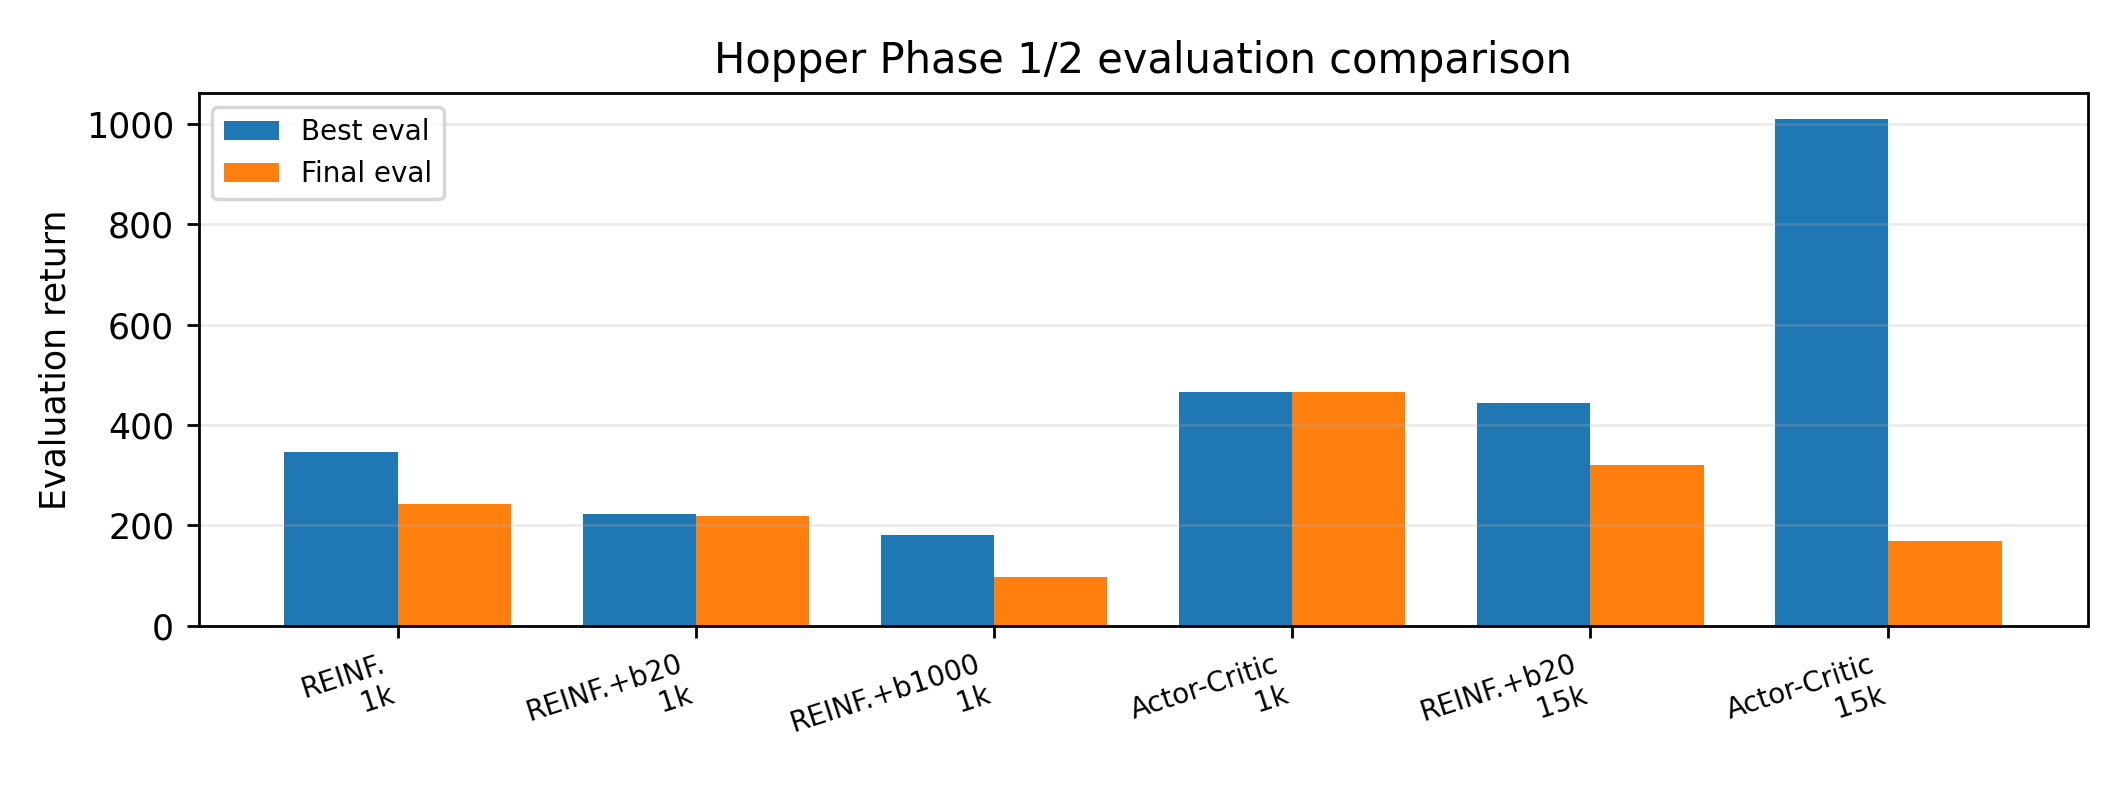
\includegraphics[width=\linewidth]{figures/hopper_phase12_eval.png}
\caption{Hopper evaluation return for all methods. Actor-Critic reaches the highest values but its 15k run degrades at the end; REINFORCE with baseline 20 provides the most stable long-run result.}
\label{fig:hopper_eval}
\end{figure}

\begin{figure}[t]
\centering
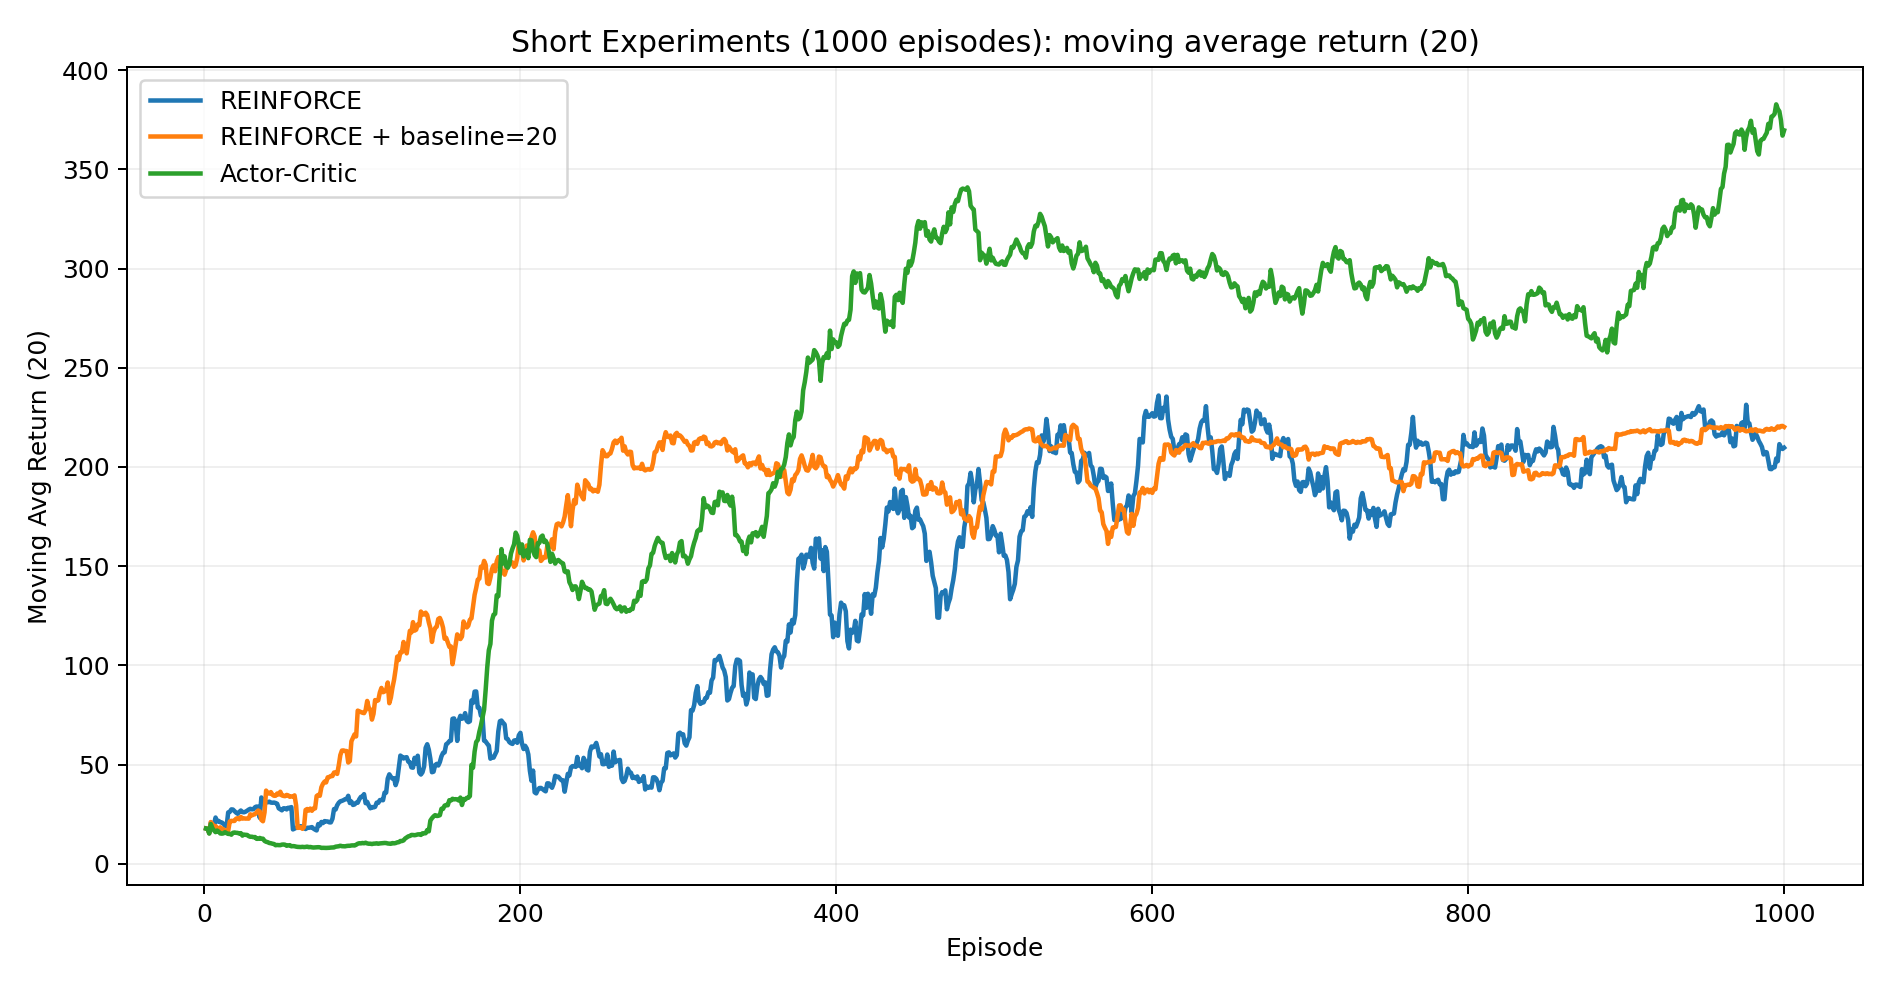
\includegraphics[width=\linewidth]{figures/hopper_1000_learning_curve.png}
\caption{Hopper training curves for the 1000-episode runs. Actor-Critic converges faster and reaches higher values, reflecting the reduced variance from step-level critic feedback.}
\label{fig:hopper_curve}
\end{figure}

\subsection{PandaPush: PPO vs SAC at 100k timesteps}

Before the 500k experiments, we compare PPO and SAC at 100k timesteps to select the algorithm for domain randomisation. The comparison is summarised in Table~\ref{tab:100k} for the key \sourcetarget transfer case. SAC achieves mean return $-3.26$ and success rate 0.24, while PPO achieves $-3.77$ and 0.12. Figure~\ref{fig:100k} shows the success rates across all configurations. SAC's advantage is consistent on the \sourcetarget case, which is the primary criterion; the most likely explanation is that its off-policy replay buffer lets it reuse past transitions more efficiently at the same timestep budget. We therefore use SAC for all subsequent 500k experiments and domain randomisation.

\begin{table}[t]
\centering
\caption{PPO vs SAC on the \sourcetarget transfer case at 100k timesteps (50 deterministic episodes). Higher return (less negative) and higher success rate are both better.}
\label{tab:100k}
\scriptsize
\setlength{\tabcolsep}{4pt}
\begin{tabular}{lrr}
\toprule
Algorithm & Mean return & Success \\
\midrule
PPO (source $\!\to\!$ target) & $-3.77$ & 0.12 \\
SAC (source $\!\to\!$ target) & $-3.26$ & \best{0.24} \\
\bottomrule
\end{tabular}
\end{table}

\begin{figure}[t]
\centering
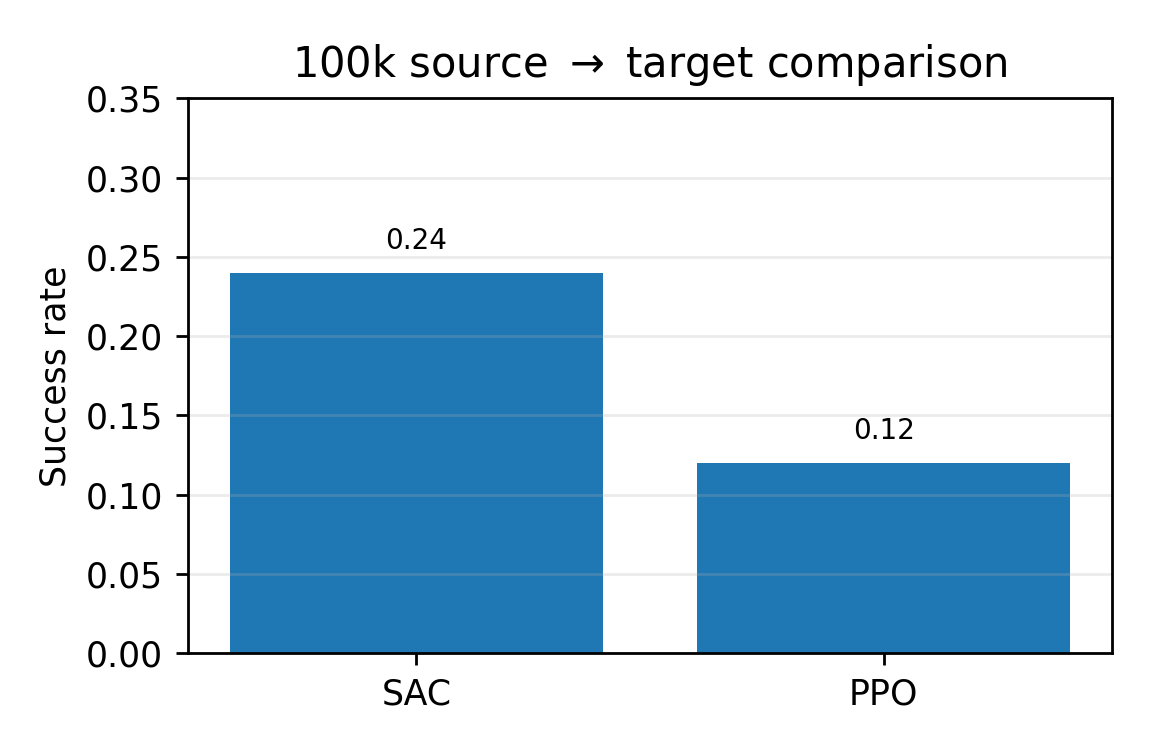
\includegraphics[width=\linewidth]{figures/phase3_100k_transfer_success.png}
\caption{PandaPush success rates for PPO and SAC at 100k timesteps. SAC is consistently superior on the key \sourcetarget case, motivating its selection for the 500k runs.}
\label{fig:100k}
\end{figure}

\subsection{PandaPush: SAC 500k baselines}

Table~\ref{tab:phase3} reports the official SAC 500k results (training seed 0, evaluation seed 1234). The \targettarget configuration reaches success rate 1.00, confirming that SAC can perfectly solve PandaPush when trained on the correct dynamics. Interestingly, the \sourcetarget result is slightly \emph{better} than \sourcesource on both metrics ($-2.073$ vs.\ $-2.276$ mean return; 0.58 vs.\ 0.52 success rate). Rather than interpreting this as evidence that the mass shift is beneficial, we attribute it to evaluation variability over 50 episodes: with such a small sample, random fluctuations in the episode outcomes can easily produce a difference of this magnitude. The gap that matters is between either lower-bound configuration (success $\le 0.58$) and the target-domain upper bound (success 1.00), which motivates the domain randomisation experiments in Phase~4. Figure~\ref{fig:phase3} provides a visual summary.

\begin{table}[t]
\centering
\caption{Official Phase~3 SAC 500k baselines (evaluation seed 1234, 50 episodes).}
\label{tab:phase3}
\scriptsize
\setlength{\tabcolsep}{3pt}
\begin{tabular}{lrrr}
\toprule
Configuration & Mean return & Std & Success \\
\midrule
\sourcesource & $-2.276$ & $2.083$ & $0.52$ \\
\sourcetarget & $-2.073$ & $1.980$ & $0.58$ \\
\targettarget & \best{$-0.475$} & $0.284$ & \best{$1.00$} \\
\bottomrule
\end{tabular}
\end{table}

\begin{figure}[t]
\centering
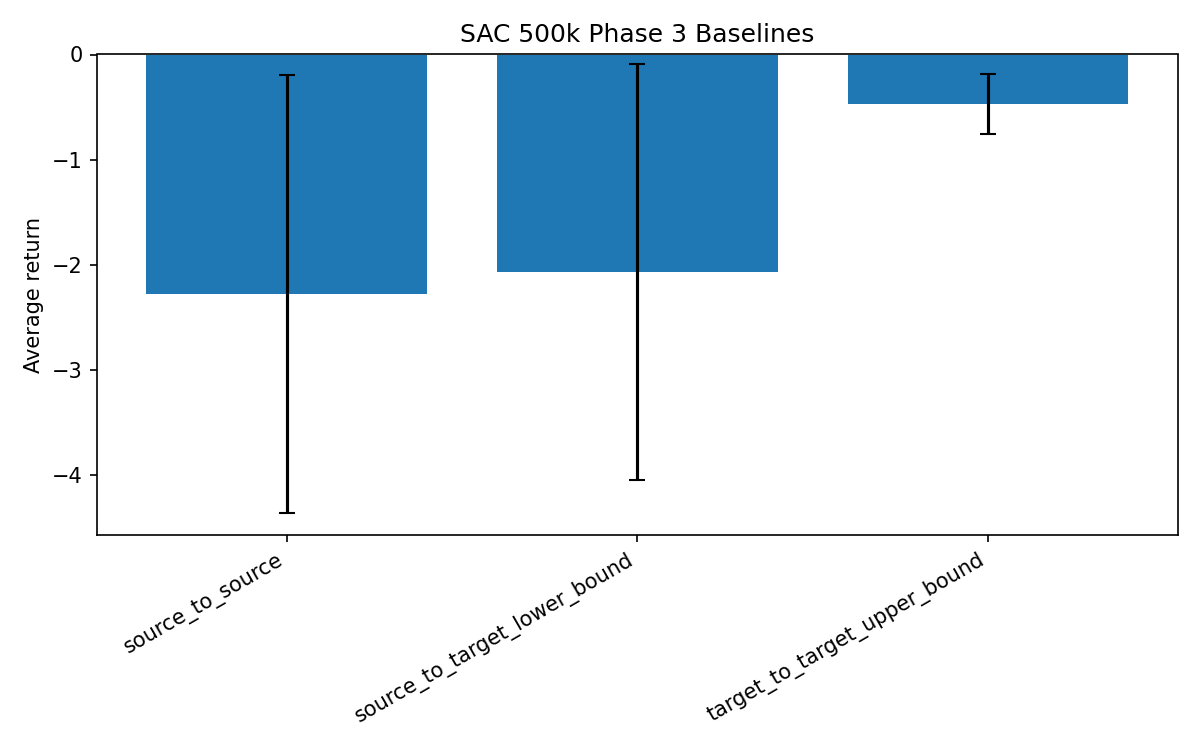
\includegraphics[width=\linewidth]{figures/phase3_sac500_eval.png}
\caption{SAC 500k evaluation results across all three transfer configurations. The target-trained upper bound achieves perfect success; the source-trained lower bound shows the unadapted transfer gap.}
\label{fig:phase3}
\end{figure}

\subsection{Domain randomisation: UDR vs ADR}

Table~\ref{tab:dr} reports the Phase~4 results. For a fair comparison, the baseline used here was evaluated within the same experimental pipeline as UDR and ADR, rather than mixing results generated during different stages of the project. The minor difference between the two \sourcetarget baseline values (success 0.50 here vs.\ 0.58 in Table~\ref{tab:phase3}) is consistent with 50-episode evaluation variance over equivalent runs.

\begin{table}[t]
\centering
\caption{Phase~4 domain randomisation results (500k SAC, 50 deterministic episodes).}
\label{tab:dr}
\scriptsize
\setlength{\tabcolsep}{3pt}
\begin{tabular}{lrrr}
\toprule
Configuration & Mean return & Std & Success \\
\midrule
SAC \sourcetarget (baseline)      & $-2.727$ & $2.328$ & $0.50$ \\
SAC \targettarget (upper bound)   & \best{$-0.416$} & $0.236$ & \best{$1.00$} \\
\midrule
UDR \sourcesource & $-0.491$ & $0.549$ & $0.98$ \\
UDR \sourcetarget & $-0.502$ & $0.420$ & \best{$1.00$} \\
\midrule
ADR \sourcesource & $-1.883$ & $1.795$ & $0.68$ \\
ADR \sourcetarget & $-1.920$ & $1.893$ & $0.66$ \\
\bottomrule
\end{tabular}
\end{table}

\begin{figure}[t]
  \centering
  \begin{subfigure}[b]{0.48\linewidth}
    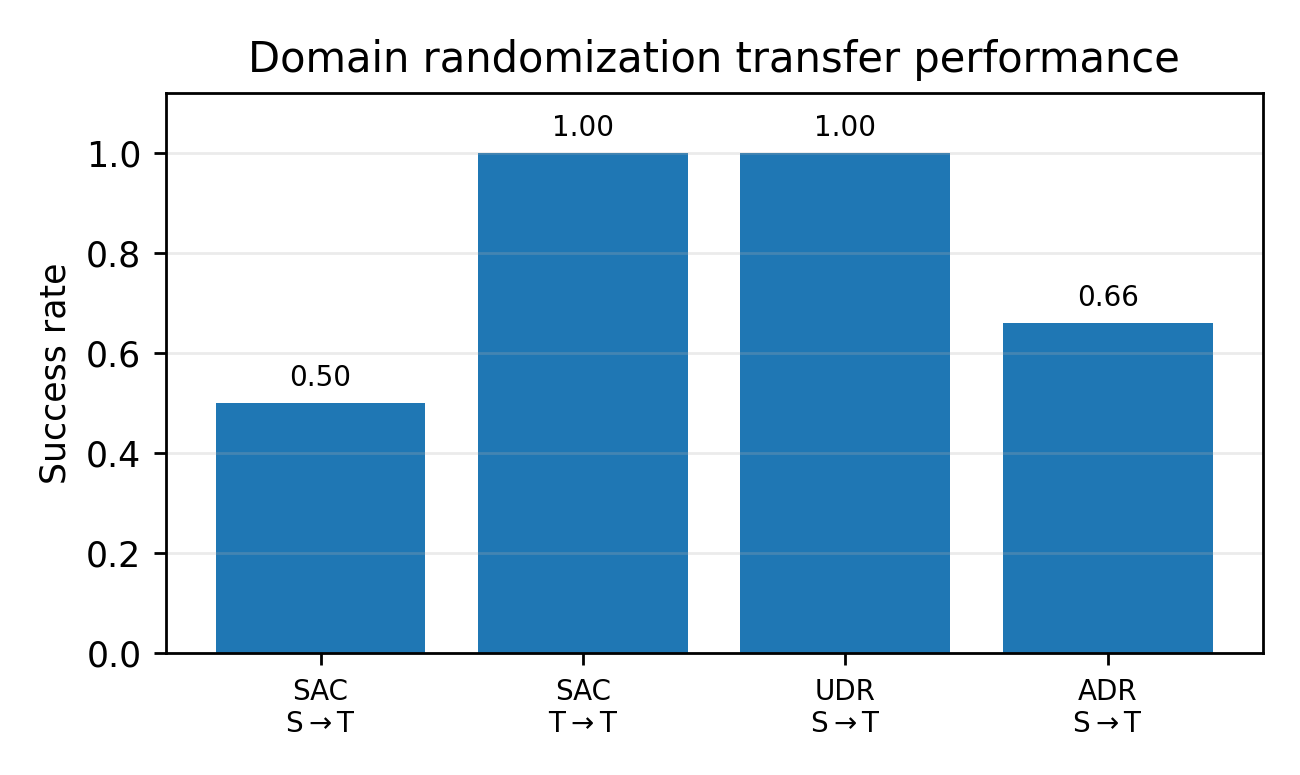
\includegraphics[width=\linewidth]{figures/phase4_dr_success.png}
    \caption{Success rates.}
    \label{fig:dr_success}
  \end{subfigure}\hfill
  \begin{subfigure}[b]{0.48\linewidth}
    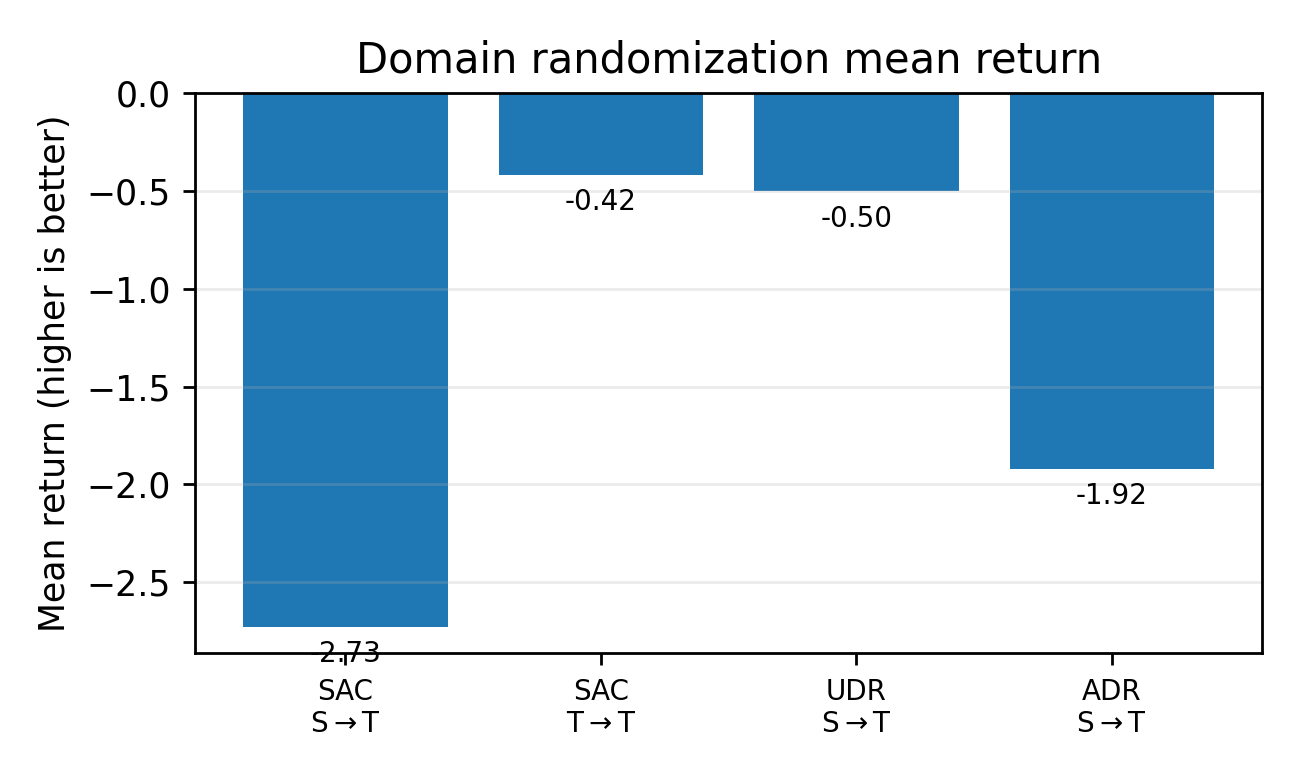
\includegraphics[width=\linewidth]{figures/phase4_dr_return.png}
    \caption{Mean returns.}
    \label{fig:dr_return}
  \end{subfigure}
  \caption{Phase~4 domain randomisation results. UDR fully closes the transfer gap in success rate and achieves a mean return close to the upper bound; ADR achieves partial improvement on both metrics.}
  \label{fig:dr}
\end{figure}

UDR is the strongest method. It raises \sourcetarget success from 0.50 to 1.00 and achieves mean return $-0.50$, very close to the upper-bound value of $-0.42$. The UDR \sourcesource result (success 0.98) confirms that the policy is also near-perfect in the source domain, demonstrating that training on a wide mass distribution does not hurt performance on the nominal source mass. ADR also improves over the baseline (0.50~$\to$~0.66 for \sourcetarget), but remains substantially weaker than UDR. Notably, ADR \sourcetarget (0.66) is slightly lower than ADR \sourcesource (0.68), suggesting that the curriculum did not adequately cover the target mass region during the available training budget.

% ----------------------------------------------------------------
\section{Discussion}
\label{sec:disc}
% ----------------------------------------------------------------

\textbf{UDR versus ADR.}
The key to UDR's success is that it uses a \emph{broad} mass range rather than a narrow distribution centred on the target mass. The range was chosen to reflect plausible variation around the source domain without assuming any prior knowledge of the exact target value. Because the target mass falls comfortably within this range, the agent encounters it routinely during training and does not treat it as an out-of-distribution case at evaluation time. ADR, by contrast, must \emph{earn} coverage of the target region through a self-paced curriculum. If the success threshold is set too conservatively, or the training budget runs out before the boundaries reach $m_t$, the policy simply never encounters the hardest transfer conditions. Our results are consistent with this failure mode: ADR \sourcesource and \sourcetarget both end up around 0.67, nearly indistinguishable, suggesting the curriculum had not yet expanded far enough to make the target mass genuinely challenging. A more thorough ADR study would tune the boundary expansion rate and success threshold, or run multiple seeds to separate algorithm behaviour from single-run variance.

\textbf{Actor-Critic instability on Hopper.}
The 15k Actor-Critic run (peak 1010.4, final 168.0) is a good illustration of a known failure mode. Early in training, the critic provides step-level advantage estimates that are low-variance and speed up the actor's progress considerably. The problem is that as the policy improves and visits new states, the critic's coverage lags behind. If bootstrapping error accumulates in these poorly-covered regions, the advantage estimates become unreliable, and a single bad update can destroy a policy that took thousands of episodes to build. REINFORCE with baseline 20, despite being noisier per update, avoids this because its gradient always comes from the actual return rather than a learned approximation. The $b=20$ vs $b=1000$ comparison also confirms a known practical rule: the baseline should be close to the expected return, not arbitrarily large---$b=1000$ sits far above early returns, which causes most advantages to be negative and effectively inverts the learning signal for the first several hundred episodes.

\textbf{Limitations.}
The most significant constraint is the use of a single training seed throughout (seed 42 for Hopper, seed 0 for PandaPush). With one run per configuration it is impossible to know how much of the observed differences are genuine algorithmic effects versus luck of initialisation. Proper statistical comparisons would require multiple seeds and reported standard errors. Beyond that, the entire study is sim-to-sim: the ``target'' is still a simulator, and a physical robot would introduce additional sources of error---sensor noise, motor backlash, control latency---that are absent here. Finally, domain randomisation was applied only to cube mass. In a real transfer scenario one would likely need to randomise friction, contact geometry, and actuator gains as well; restricting to a single parameter limits the generality of the conclusions.

% ----------------------------------------------------------------
\section{Conclusion}
% ----------------------------------------------------------------

We implemented three policy-gradient algorithms from scratch on Hopper and benchmarked PPO and SAC on PandaPush using Stable-Baselines3. Actor-Critic was the best-performing Hopper method at 1000 episodes. On PandaPush, SAC was consistently stronger than PPO at 100k timesteps and was used for all subsequent 500k experiments. The domain randomisation results are the most notable outcome of the project: UDR raised source-to-target success from 0.50 to 1.00, fully matching the target upper bound while never training on target dynamics; ADR improved over the unadapted baseline (0.50~$\to$~0.66) but did not match UDR in our run. Overall, these findings confirm that training on a distribution of dynamics, even over a single physical parameter, can be enough to close a substantial transfer gap. Future work should extend randomisation to multiple parameters, evaluate with multiple seeds, and validate on physical hardware.

{
\footnotesize
\begin{thebibliography}{99}
\bibitem{sutton2018reinforcement} R.~S. Sutton and A.~G. Barto. \emph{Reinforcement Learning: An Introduction}. MIT Press, 2nd edition, 2018.
\bibitem{kober2013robotics} J.~Kober, J.~A. Bagnell, and J.~Peters. Reinforcement learning in robotics: A survey. \emph{Int.\ J.\ Robotics Research}, 32(11):1238--1274, 2013.
\bibitem{kormushev2013applications} P.~Kormushev, S.~Calinon, and D.~G. Caldwell. Reinforcement learning in robotics: Applications and real-world challenges. \emph{Robotics}, 2(3):122--148, 2013.
\bibitem{hofer2021perspectives} S.~H{\"o}fer et al. Perspectives on sim2real transfer for robotics. \emph{IEEE RA-L}, 6(3):4480--4487, 2021.
\bibitem{tobin2017domain} J.~Tobin et al. Domain randomization for transferring deep neural networks from simulation to the real world. In \emph{IROS}, 2017.
\bibitem{peng2018sim} X.~B. Peng, M.~Andrychowicz, W.~Zaremba, and P.~Abbeel. Sim-to-real transfer of robotic control with dynamics randomization. In \emph{ICRA}, 2018.
\bibitem{muratore2022robot} F.~Muratore, C.~Eilers, M.~Gienger, and J.~Peters. Robot learning from randomized simulations: A review. \emph{Frontiers in Robotics and AI}, 9, 2022.
\bibitem{akkaya2019rubiks} I.~Akkaya et al. Solving Rubik's Cube with a robot hand. \emph{arXiv:1910.07113}, 2019.
\bibitem{schulman2017ppo} J.~Schulman, F.~Wolski, P.~Dhariwal, A.~Radford, and O.~Klimov. Proximal policy optimization algorithms. \emph{arXiv:1707.06347}, 2017.
\bibitem{haarnoja2018sac} T.~Haarnoja, A.~Zhou, P.~Abbeel, and S.~Levine. Soft Actor-Critic: Off-policy maximum entropy deep RL with a stochastic actor. In \emph{ICML}, 2018.
\bibitem{raffin2021stable} A.~Raffin et al. Stable-Baselines3: Reliable RL implementations. \emph{JMLR}, 22(268):1--8, 2021.
\bibitem{todorov2012mujoco} E.~Todorov, T.~Erez, and Y.~Tassa. MuJoCo: A physics engine for model-based control. In \emph{IROS}, 2012.
\bibitem{gallouedec2021pandagym} Q.~Gallou{\'e}dec, N.~Cazin, E.~Dellandr{\'e}a, and L.~Chen. panda-gym: Open-source goal-conditioned environments for robotic learning, 2021.
\end{thebibliography}
}

\end{document}
